\documentclass[1p]{elsarticle_modified}
%\bibliographystyle{elsarticle-num}

%\usepackage[colorlinks]{hyperref}
%\usepackage{abbrmath_seonhwa} %\Abb, \Ascr, \Acal ,\Abf, \Afrak
\usepackage{amsfonts}
\usepackage{amssymb}
\usepackage{amsmath}
\usepackage{amsthm}
\usepackage{scalefnt}
\usepackage{amsbsy}
\usepackage{kotex}
\usepackage{caption}
\usepackage{subfig}
\usepackage{color}
\usepackage{graphicx}
\usepackage{xcolor} %% white, black, red, green, blue, cyan, magenta, yellow
\usepackage{float}
\usepackage{setspace}
\usepackage{hyperref}

\usepackage{tikz}
\usetikzlibrary{arrows}

\usepackage{multirow}
\usepackage{array} % fixed length table
\usepackage{hhline}

%%%%%%%%%%%%%%%%%%%%%
\makeatletter
\renewcommand*\env@matrix[1][\arraystretch]{%
	\edef\arraystretch{#1}%
	\hskip -\arraycolsep
	\let\@ifnextchar\new@ifnextchar
	\array{*\c@MaxMatrixCols c}}
\makeatother %https://tex.stackexchange.com/questions/14071/how-can-i-increase-the-line-spacing-in-a-matrix
%%%%%%%%%%%%%%%

\usepackage[normalem]{ulem}

\newcommand{\msout}[1]{\ifmmode\text{\sout{\ensuremath{#1}}}\else\sout{#1}\fi}
%SOURCE: \msout is \stkout macro in https://tex.stackexchange.com/questions/20609/strikeout-in-math-mode

\newcommand{\cancel}[1]{
	\ifmmode
	{\color{red}\msout{#1}}
	\else
	{\color{red}\sout{#1}}
	\fi
}

\newcommand{\add}[1]{
	{\color{blue}\uwave{#1}}
}

\newcommand{\replace}[2]{
	\ifmmode
	{\color{red}\msout{#1}}{\color{blue}\uwave{#2}}
	\else
	{\color{red}\sout{#1}}{\color{blue}\uwave{#2}}
	\fi
}

\newcommand{\Sol}{\mathcal{S}} %segment
\newcommand{\D}{D} %diagram
\newcommand{\A}{\mathcal{A}} %arc


%%%%%%%%%%%%%%%%%%%%%%%%%%%%%5 test

\def\sl{\operatorname{\textup{SL}}(2,\Cbb)}
\def\psl{\operatorname{\textup{PSL}}(2,\Cbb)}
\def\quan{\mkern 1mu \triangleright \mkern 1mu}

\theoremstyle{definition}
\newtheorem{thm}{Theorem}[section]
\newtheorem{prop}[thm]{Proposition}
\newtheorem{lem}[thm]{Lemma}
\newtheorem{ques}[thm]{Question}
\newtheorem{cor}[thm]{Corollary}
\newtheorem{defn}[thm]{Definition}
\newtheorem{exam}[thm]{Example}
\newtheorem{rmk}[thm]{Remark}
\newtheorem{alg}[thm]{Algorithm}

\newcommand{\I}{\sqrt{-1}}
\begin{document}

%\begin{frontmatter}
%
%\title{Boundary parabolic representations of knots up to 8 crossings}
%
%%% Group authors per affiliation:
%\author{Yunhi Cho} 
%\address{Department of Mathematics, University of Seoul, Seoul, Korea}
%\ead{yhcho@uos.ac.kr}
%
%
%\author{Seonhwa Kim} %\fnref{s_kim}}
%\address{Center for Geometry and Physics, Institute for Basic Science, Pohang, 37673, Korea}
%\ead{ryeona17@ibs.re.kr}
%
%\author{Hyuk Kim}
%\address{Department of Mathematical Sciences, Seoul National University, Seoul 08826, Korea}
%\ead{hyukkim@snu.ac.kr}
%
%\author{Seokbeom Yoon}
%\address{Department of Mathematical Sciences, Seoul National University, Seoul, 08826,  Korea}
%\ead{sbyoon15@snu.ac.kr}
%
%\begin{abstract}
%We find all boundary parabolic representation of knots up to 8 crossings.
%
%\end{abstract}
%\begin{keyword}
%    \MSC[2010] 57M25 
%\end{keyword}
%
%\end{frontmatter}

%\linenumbers
%\tableofcontents
%
\newcommand\colored[1]{\textcolor{white}{\rule[-0.35ex]{0.8em}{1.4ex}}\kern-0.8em\color{red} #1}%
%\newcommand\colored[1]{\textcolor{white}{ #1}\kern-2.17ex	\textcolor{white}{ #1}\kern-1.81ex	\textcolor{white}{ #1}\kern-2.15ex\color{red}#1	}

{\Large $\underline{12a_{1091}~(K12a_{1091})}$}

\setlength{\tabcolsep}{10pt}
\renewcommand{\arraystretch}{1.6}
\vspace{1cm}\begin{tabular}{m{100pt}>{\centering\arraybackslash}m{274pt}}
\multirow{5}{120pt}{
	\centering
	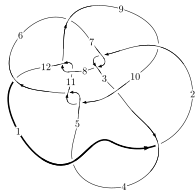
\includegraphics[width=112pt]{../../../GIT/diagram.site/Diagrams/png/1892_12a_1091.png}\\
\ \ \ A knot diagram\footnotemark}&
\allowdisplaybreaks
\textbf{Linearized knot diagam} \\
\cline{2-2}
 &
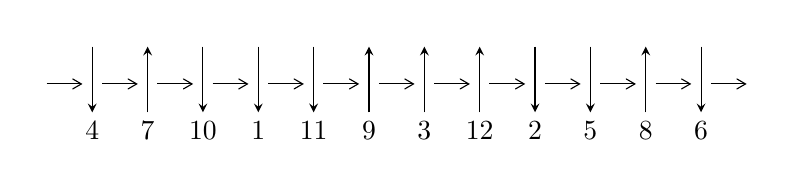
\begin{tikzpicture}[x=20pt, y=17pt]
	% nodes
	\node (C0) at (0, 0) {};
	\node (C1) at (1, 0) {};
	\node (C1U) at (1, +1) {};
	\node (C1D) at (1, -1) {4};

	\node (C2) at (2, 0) {};
	\node (C2U) at (2, +1) {};
	\node (C2D) at (2, -1) {7};

	\node (C3) at (3, 0) {};
	\node (C3U) at (3, +1) {};
	\node (C3D) at (3, -1) {10};

	\node (C4) at (4, 0) {};
	\node (C4U) at (4, +1) {};
	\node (C4D) at (4, -1) {1};

	\node (C5) at (5, 0) {};
	\node (C5U) at (5, +1) {};
	\node (C5D) at (5, -1) {11};

	\node (C6) at (6, 0) {};
	\node (C6U) at (6, +1) {};
	\node (C6D) at (6, -1) {9};

	\node (C7) at (7, 0) {};
	\node (C7U) at (7, +1) {};
	\node (C7D) at (7, -1) {3};

	\node (C8) at (8, 0) {};
	\node (C8U) at (8, +1) {};
	\node (C8D) at (8, -1) {12};

	\node (C9) at (9, 0) {};
	\node (C9U) at (9, +1) {};
	\node (C9D) at (9, -1) {2};

	\node (C10) at (10, 0) {};
	\node (C10U) at (10, +1) {};
	\node (C10D) at (10, -1) {5};

	\node (C11) at (11, 0) {};
	\node (C11U) at (11, +1) {};
	\node (C11D) at (11, -1) {8};

	\node (C12) at (12, 0) {};
	\node (C12U) at (12, +1) {};
	\node (C12D) at (12, -1) {6};
	\node (C13) at (13, 0) {};

	% arrows
	\draw[->,>={angle 60}]
	(C0) edge (C1) (C1) edge (C2) (C2) edge (C3) (C3) edge (C4) (C4) edge (C5) (C5) edge (C6) (C6) edge (C7) (C7) edge (C8) (C8) edge (C9) (C9) edge (C10) (C10) edge (C11) (C11) edge (C12) (C12) edge (C13) ;	\draw[->,>=stealth]
	(C1U) edge (C1D) (C2D) edge (C2U) (C3U) edge (C3D) (C4U) edge (C4D) (C5U) edge (C5D) (C6D) edge (C6U) (C7D) edge (C7U) (C8D) edge (C8U) (C9U) edge (C9D) (C10U) edge (C10D) (C11D) edge (C11U) (C12U) edge (C12D) ;
	\end{tikzpicture} \\
\hhline{~~} \\& 
\textbf{Solving Sequence} \\ \cline{2-2} 
 &
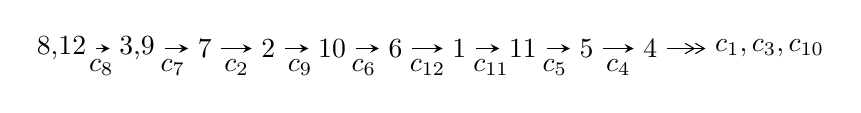
\begin{tikzpicture}[x=23pt, y=7pt]
	% node
	\node (A0) at (-1/8, 0) {8,12};
	\node (A1) at (17/16, 0) {3,9};
	\node (A2) at (17/8, 0) {7};
	\node (A3) at (25/8, 0) {2};
	\node (A4) at (33/8, 0) {10};
	\node (A5) at (41/8, 0) {6};
	\node (A6) at (49/8, 0) {1};
	\node (A7) at (57/8, 0) {11};
	\node (A8) at (65/8, 0) {5};
	\node (A9) at (73/8, 0) {4};
	\node (C1) at (1/2, -1) {$c_{8}$};
	\node (C2) at (13/8, -1) {$c_{7}$};
	\node (C3) at (21/8, -1) {$c_{2}$};
	\node (C4) at (29/8, -1) {$c_{9}$};
	\node (C5) at (37/8, -1) {$c_{6}$};
	\node (C6) at (45/8, -1) {$c_{12}$};
	\node (C7) at (53/8, -1) {$c_{11}$};
	\node (C8) at (61/8, -1) {$c_{5}$};
	\node (C9) at (69/8, -1) {$c_{4}$};
	\node (A10) at (11, 0) {$c_{1},c_{3},c_{10}$};

	% edge
	\draw[->,>=stealth]	
	(A0) edge (A1) (A1) edge (A2) (A2) edge (A3) (A3) edge (A4) (A4) edge (A5) (A5) edge (A6) (A6) edge (A7) (A7) edge (A8) (A8) edge (A9) ;
	\draw[->>,>={angle 60}]	
	(A9) edge (A10);
\end{tikzpicture} \\ 

\end{tabular} \\

\footnotetext{
The image of knot diagram is generated by the software ``\textbf{Draw programme}" developed by Andrew Bartholomew(\url{http://www.layer8.co.uk/maths/draw/index.htm\#Running-draw}), where we modified some parts for our purpose(\url{https://github.com/CATsTAILs/LinksPainter}).
}\phantom \\ \newline 
\centering \textbf{Ideals for irreducible components\footnotemark of $X_{\text{par}}$} 
 
\begin{align*}
I^u_{1}&=\langle 
-6.39310\times10^{837} u^{160}+4.58819\times10^{837} u^{159}+\cdots+1.25873\times10^{837} b+1.99542\times10^{842},\\
\phantom{I^u_{1}}&\phantom{= \langle  }1.45185\times10^{842} u^{160}-7.32509\times10^{841} u^{159}+\cdots+2.86374\times10^{841} a-5.38127\times10^{846},\\
\phantom{I^u_{1}}&\phantom{= \langle  }u^{161}-43 u^{159}+\cdots+23192 u-22751\rangle \\
I^u_{2}&=\langle 
-1.30052\times10^{27} u^{42}+5.58534\times10^{27} u^{41}+\cdots+5.17611\times10^{24} b-1.73362\times10^{27},\\
\phantom{I^u_{2}}&\phantom{= \langle  }-5.05339\times10^{27} u^{42}+2.24625\times10^{28} u^{41}+\cdots+5.17611\times10^{24} a-8.77138\times10^{27},\;u^{43}-5 u^{42}+\cdots+9 u-1\rangle \\
\\
\end{align*}
\raggedright * 2 irreducible components of $\dim_{\mathbb{C}}=0$, with total 204 representations.\\
\footnotetext{All coefficients of polynomials are rational numbers. But the coefficients are sometimes approximated in decimal forms when there is not enough margin.}
\newpage
\renewcommand{\arraystretch}{1}
\centering \section*{I. $I^u_{1}= \langle -6.39\times10^{837} u^{160}+4.59\times10^{837} u^{159}+\cdots+1.26\times10^{837} b+2.00\times10^{842},\;1.45\times10^{842} u^{160}-7.33\times10^{841} u^{159}+\cdots+2.86\times10^{841} a-5.38\times10^{846},\;u^{161}-43 u^{159}+\cdots+23192 u-22751 \rangle$}
\flushleft \textbf{(i) Arc colorings}\\
\begin{tabular}{m{7pt} m{180pt} m{7pt} m{180pt} }
\flushright $a_{8}=$&$\begin{pmatrix}1\\0\end{pmatrix}$ \\
\flushright $a_{12}=$&$\begin{pmatrix}0\\u\end{pmatrix}$ \\
\flushright $a_{3}=$&$\begin{pmatrix}-5.06979 u^{160}+2.55788 u^{159}+\cdots-468625. u+187911.\\5.07901 u^{160}-3.64509 u^{159}+\cdots+375636. u-158527.\end{pmatrix}$ \\
\flushright $a_{9}=$&$\begin{pmatrix}1\\- u^2\end{pmatrix}$ \\
\flushright $a_{7}=$&$\begin{pmatrix}10.6826 u^{160}-9.77082 u^{159}+\cdots+576831. u-269285.\\-24.6702 u^{160}+21.3731 u^{159}+\cdots-1.39803\times10^{6} u+645587.\end{pmatrix}$ \\
\flushright $a_{2}=$&$\begin{pmatrix}1.12700 u^{160}-6.54266 u^{159}+\cdots-510744. u+142501.\\1.25989 u^{160}+0.372663 u^{159}+\cdots+244271. u-82982.0\end{pmatrix}$ \\
\flushright $a_{10}=$&$\begin{pmatrix}-80.0417 u^{160}+75.0777 u^{159}+\cdots-4.05107\times10^{6} u+1.94173\times10^{6}\\28.1384 u^{160}-23.4524 u^{159}+\cdots+1.66699\times10^{6} u-759659.\end{pmatrix}$ \\
\flushright $a_{6}=$&$\begin{pmatrix}26.3009 u^{160}-22.6628 u^{159}+\cdots+1.50521\times10^{6} u-692577.\\-35.0998 u^{160}+29.6020 u^{159}+\cdots-2.05235\times10^{6} u+938893.\end{pmatrix}$ \\
\flushright $a_{1}=$&$\begin{pmatrix}74.7417 u^{160}-62.5278 u^{159}+\cdots+4.47416\times10^{6} u-2.02663\times10^{6}\\-45.8026 u^{160}+37.7780 u^{159}+\cdots-2.80124\times10^{6} u+1.25943\times10^{6}\end{pmatrix}$ \\
\flushright $a_{11}=$&$\begin{pmatrix}- u\\u\end{pmatrix}$ \\
\flushright $a_{5}=$&$\begin{pmatrix}21.0485 u^{160}-18.9227 u^{159}+\cdots+1.14409\times10^{6} u-534703.\\-29.8474 u^{160}+25.8619 u^{159}+\cdots-1.69123\times10^{6} u+781019.\end{pmatrix}$ \\
\flushright $a_{4}=$&$\begin{pmatrix}-23.3510 u^{160}+15.7838 u^{159}+\cdots-1.78107\times10^{6} u+747855.\\-11.4670 u^{160}+12.3883 u^{159}+\cdots-382645. u+221297.\end{pmatrix}$\\&\end{tabular}
\flushleft \textbf{(ii) Obstruction class $= -1$}\\~\\
\flushleft \textbf{(iii) Cusp Shapes $= -357.352 u^{160}+338.730 u^{159}+\cdots-1.76787\times10^{7} u+8.55098\times10^{6}$}\\~\\
\newpage\renewcommand{\arraystretch}{1}
\flushleft \textbf{(iv) u-Polynomials at the component}\newline \\
\begin{tabular}{m{50pt}|m{274pt}}
Crossings & \hspace{64pt}u-Polynomials at each crossing \\
\hline $$\begin{aligned}c_{1},c_{4}\end{aligned}$$&$\begin{aligned}
&u^{161}-6 u^{160}+\cdots-60405 u+2525
\end{aligned}$\\
\hline $$\begin{aligned}c_{2},c_{7}\end{aligned}$$&$\begin{aligned}
&u^{161}+u^{160}+\cdots+62875 u+20690
\end{aligned}$\\
\hline $$\begin{aligned}c_{3}\end{aligned}$$&$\begin{aligned}
&u^{161}+u^{160}+\cdots+6424407 u-1081037
\end{aligned}$\\
\hline $$\begin{aligned}c_{5},c_{10}\end{aligned}$$&$\begin{aligned}
&u^{161}-5 u^{160}+\cdots-34377 u-24287
\end{aligned}$\\
\hline $$\begin{aligned}c_{6}\end{aligned}$$&$\begin{aligned}
&u^{161}+4 u^{160}+\cdots+209706558586 u+17633051719
\end{aligned}$\\
\hline $$\begin{aligned}c_{8},c_{11}\end{aligned}$$&$\begin{aligned}
&u^{161}-43 u^{159}+\cdots+23192 u+22751
\end{aligned}$\\
\hline $$\begin{aligned}c_{9}\end{aligned}$$&$\begin{aligned}
&u^{161}+5 u^{160}+\cdots+5900566245 u-806431049
\end{aligned}$\\
\hline $$\begin{aligned}c_{12}\end{aligned}$$&$\begin{aligned}
&u^{161}+2 u^{160}+\cdots+297854463 u-20528044
\end{aligned}$\\
\hline
\end{tabular}\\~\\
\newpage\renewcommand{\arraystretch}{1}
\flushleft \textbf{(v) Riley Polynomials at the component}\newline \\
\begin{tabular}{m{50pt}|m{274pt}}
Crossings & \hspace{64pt}Riley Polynomials at each crossing \\
\hline $$\begin{aligned}c_{1},c_{4}\end{aligned}$$&$\begin{aligned}
&y^{161}+104 y^{160}+\cdots-44901925 y-6375625
\end{aligned}$\\
\hline $$\begin{aligned}c_{2},c_{7}\end{aligned}$$&$\begin{aligned}
&y^{161}-95 y^{160}+\cdots+56848574785 y-428076100
\end{aligned}$\\
\hline $$\begin{aligned}c_{3}\end{aligned}$$&$\begin{aligned}
&y^{161}+13 y^{160}+\cdots-81817610068445 y-1168640995369
\end{aligned}$\\
\hline $$\begin{aligned}c_{5},c_{10}\end{aligned}$$&$\begin{aligned}
&y^{161}-71 y^{160}+\cdots-8324930855 y-589858369
\end{aligned}$\\
\hline $$\begin{aligned}c_{6}\end{aligned}$$&$\begin{aligned}
&y^{161}-44 y^{160}+\cdots+4.98\times10^{21} y-3.11\times10^{20}
\end{aligned}$\\
\hline $$\begin{aligned}c_{8},c_{11}\end{aligned}$$&$\begin{aligned}
&y^{161}-86 y^{160}+\cdots+30379536528 y-517608001
\end{aligned}$\\
\hline $$\begin{aligned}c_{9}\end{aligned}$$&$\begin{aligned}
&y^{161}+29 y^{160}+\cdots-3.95\times10^{19} y-6.50\times10^{17}
\end{aligned}$\\
\hline $$\begin{aligned}c_{12}\end{aligned}$$&$\begin{aligned}
&y^{161}+36 y^{160}+\cdots-32685559262828287 y-421400590465936
\end{aligned}$\\
\hline
\end{tabular}\\~\\
\newpage\flushleft \textbf{(vi) Complex Volumes and Cusp Shapes}
$$\begin{array}{c|c|c}  
\text{Solutions to }I^u_{1}& \I (\text{vol} + \sqrt{-1}CS) & \text{Cusp shape}\\
 \hline 
\begin{aligned}
u &= -0.950374 + 0.325702 I \\
a &= \phantom{-}0.393996 - 0.385326 I \\
b &= \phantom{-}0.169698 + 0.056372 I\end{aligned}
 & \phantom{-}1.60788 - 1.20779 I & \phantom{-0.000000 } 0 \\ \hline\begin{aligned}
u &= -0.950374 - 0.325702 I \\
a &= \phantom{-}0.393996 + 0.385326 I \\
b &= \phantom{-}0.169698 - 0.056372 I\end{aligned}
 & \phantom{-}1.60788 + 1.20779 I & \phantom{-0.000000 } 0 \\ \hline\begin{aligned}
u &= -0.072510 + 0.991759 I \\
a &= -0.559105 - 0.563435 I \\
b &= \phantom{-}1.205640 - 0.484119 I\end{aligned}
 & \phantom{-}6.47296 - 7.82720 I & \phantom{-0.000000 } 0 \\ \hline\begin{aligned}
u &= -0.072510 - 0.991759 I \\
a &= -0.559105 + 0.563435 I \\
b &= \phantom{-}1.205640 + 0.484119 I\end{aligned}
 & \phantom{-}6.47296 + 7.82720 I & \phantom{-0.000000 } 0 \\ \hline\begin{aligned}
u &= -0.993352 + 0.197972 I \\
a &= \phantom{-}2.56889 + 0.55840 I \\
b &= -1.30419 + 0.69007 I\end{aligned}
 & \phantom{-}0.61248 - 4.81440 I & \phantom{-0.000000 } 0 \\ \hline\begin{aligned}
u &= -0.993352 - 0.197972 I \\
a &= \phantom{-}2.56889 - 0.55840 I \\
b &= -1.30419 - 0.69007 I\end{aligned}
 & \phantom{-}0.61248 + 4.81440 I & \phantom{-0.000000 } 0 \\ \hline\begin{aligned}
u &= \phantom{-}0.902874 + 0.463441 I \\
a &= \phantom{-}1.336050 - 0.193210 I \\
b &= -0.871684 - 0.901749 I\end{aligned}
 & -0.08463 + 5.13600 I & \phantom{-0.000000 } 0 \\ \hline\begin{aligned}
u &= \phantom{-}0.902874 - 0.463441 I \\
a &= \phantom{-}1.336050 + 0.193210 I \\
b &= -0.871684 + 0.901749 I\end{aligned}
 & -0.08463 - 5.13600 I & \phantom{-0.000000 } 0 \\ \hline\begin{aligned}
u &= -0.955013 + 0.229039 I \\
a &= -2.93997 - 0.42458 I \\
b &= \phantom{-}1.50313 - 0.49893 I\end{aligned}
 & \phantom{-}3.79930 - 8.84455 I & \phantom{-0.000000 } 0 \\ \hline\begin{aligned}
u &= -0.955013 - 0.229039 I \\
a &= -2.93997 + 0.42458 I \\
b &= \phantom{-}1.50313 + 0.49893 I\end{aligned}
 & \phantom{-}3.79930 + 8.84455 I & \phantom{-0.000000 } 0\\
 \hline 
 \end{array}$$\newpage$$\begin{array}{c|c|c}  
\text{Solutions to }I^u_{1}& \I (\text{vol} + \sqrt{-1}CS) & \text{Cusp shape}\\
 \hline 
\begin{aligned}
u &= -0.173656 + 0.965528 I \\
a &= \phantom{-}0.467423 + 0.277205 I \\
b &= -1.156730 + 0.326183 I\end{aligned}
 & \phantom{-}1.90577 - 4.13490 I & \phantom{-0.000000 } 0 \\ \hline\begin{aligned}
u &= -0.173656 - 0.965528 I \\
a &= \phantom{-}0.467423 - 0.277205 I \\
b &= -1.156730 - 0.326183 I\end{aligned}
 & \phantom{-}1.90577 + 4.13490 I & \phantom{-0.000000 } 0 \\ \hline\begin{aligned}
u &= \phantom{-}0.363651 + 0.909552 I \\
a &= \phantom{-}0.282299 - 0.406949 I \\
b &= -0.623074 - 0.340925 I\end{aligned}
 & -1.77610 - 2.50851 I & \phantom{-0.000000 } 0 \\ \hline\begin{aligned}
u &= \phantom{-}0.363651 - 0.909552 I \\
a &= \phantom{-}0.282299 + 0.406949 I \\
b &= -0.623074 + 0.340925 I\end{aligned}
 & -1.77610 + 2.50851 I & \phantom{-0.000000 } 0 \\ \hline\begin{aligned}
u &= -0.133671 + 0.967135 I \\
a &= \phantom{-}0.363269 + 0.968622 I \\
b &= -0.060760 + 1.024230 I\end{aligned}
 & -0.48025 + 8.06330 I & \phantom{-0.000000 } 0 \\ \hline\begin{aligned}
u &= -0.133671 - 0.967135 I \\
a &= \phantom{-}0.363269 - 0.968622 I \\
b &= -0.060760 - 1.024230 I\end{aligned}
 & -0.48025 - 8.06330 I & \phantom{-0.000000 } 0 \\ \hline\begin{aligned}
u &= -0.923789 + 0.443969 I \\
a &= \phantom{-}0.26507 + 1.48143 I \\
b &= -0.951484 - 0.034762 I\end{aligned}
 & \phantom{-}4.76381 + 0.13098 I & \phantom{-0.000000 } 0 \\ \hline\begin{aligned}
u &= -0.923789 - 0.443969 I \\
a &= \phantom{-}0.26507 - 1.48143 I \\
b &= -0.951484 + 0.034762 I\end{aligned}
 & \phantom{-}4.76381 - 0.13098 I & \phantom{-0.000000 } 0 \\ \hline\begin{aligned}
u &= \phantom{-}0.794847 + 0.656611 I \\
a &= \phantom{-}0.210662 + 0.974229 I \\
b &= -0.875222 + 0.010488 I\end{aligned}
 & \phantom{-}6.86027 + 2.36778 I & \phantom{-0.000000 } 0 \\ \hline\begin{aligned}
u &= \phantom{-}0.794847 - 0.656611 I \\
a &= \phantom{-}0.210662 - 0.974229 I \\
b &= -0.875222 - 0.010488 I\end{aligned}
 & \phantom{-}6.86027 - 2.36778 I & \phantom{-0.000000 } 0\\
 \hline 
 \end{array}$$\newpage$$\begin{array}{c|c|c}  
\text{Solutions to }I^u_{1}& \I (\text{vol} + \sqrt{-1}CS) & \text{Cusp shape}\\
 \hline 
\begin{aligned}
u &= \phantom{-}0.990904 + 0.328079 I \\
a &= \phantom{-}0.276707 + 0.562545 I \\
b &= -0.696982 + 0.658755 I\end{aligned}
 & -2.70689 + 1.93033 I & \phantom{-0.000000 } 0 \\ \hline\begin{aligned}
u &= \phantom{-}0.990904 - 0.328079 I \\
a &= \phantom{-}0.276707 - 0.562545 I \\
b &= -0.696982 - 0.658755 I\end{aligned}
 & -2.70689 - 1.93033 I & \phantom{-0.000000 } 0 \\ \hline\begin{aligned}
u &= \phantom{-}0.955110 + 0.432923 I \\
a &= -0.730781 - 0.042302 I \\
b &= \phantom{-}0.519570 + 0.834793 I\end{aligned}
 & \phantom{-}0.31187 + 3.75114 I & \phantom{-0.000000 } 0 \\ \hline\begin{aligned}
u &= \phantom{-}0.955110 - 0.432923 I \\
a &= -0.730781 + 0.042302 I \\
b &= \phantom{-}0.519570 - 0.834793 I\end{aligned}
 & \phantom{-}0.31187 - 3.75114 I & \phantom{-0.000000 } 0 \\ \hline\begin{aligned}
u &= \phantom{-}1.023370 + 0.258291 I \\
a &= -0.437416 - 1.185920 I \\
b &= \phantom{-}0.685995 - 0.525139 I\end{aligned}
 & \phantom{-}1.01774 + 6.80120 I & \phantom{-0.000000 } 0 \\ \hline\begin{aligned}
u &= \phantom{-}1.023370 - 0.258291 I \\
a &= -0.437416 + 1.185920 I \\
b &= \phantom{-}0.685995 + 0.525139 I\end{aligned}
 & \phantom{-}1.01774 - 6.80120 I & \phantom{-0.000000 } 0 \\ \hline\begin{aligned}
u &= \phantom{-}0.836063 + 0.420493 I \\
a &= -1.70373 + 0.81945 I \\
b &= \phantom{-}0.969989 + 0.648626 I\end{aligned}
 & \phantom{-}1.31743 + 5.01058 I & \phantom{-0.000000 } 0 \\ \hline\begin{aligned}
u &= \phantom{-}0.836063 - 0.420493 I \\
a &= -1.70373 - 0.81945 I \\
b &= \phantom{-}0.969989 - 0.648626 I\end{aligned}
 & \phantom{-}1.31743 - 5.01058 I & \phantom{-0.000000 } 0 \\ \hline\begin{aligned}
u &= \phantom{-}0.633559 + 0.685378 I \\
a &= -0.527296 - 0.412378 I \\
b &= -0.933157 + 0.296491 I\end{aligned}
 & -3.10634 - 1.77812 I & \phantom{-0.000000 } 0 \\ \hline\begin{aligned}
u &= \phantom{-}0.633559 - 0.685378 I \\
a &= -0.527296 + 0.412378 I \\
b &= -0.933157 - 0.296491 I\end{aligned}
 & -3.10634 + 1.77812 I & \phantom{-0.000000 } 0\\
 \hline 
 \end{array}$$\newpage$$\begin{array}{c|c|c}  
\text{Solutions to }I^u_{1}& \I (\text{vol} + \sqrt{-1}CS) & \text{Cusp shape}\\
 \hline 
\begin{aligned}
u &= -1.048950 + 0.218293 I \\
a &= \phantom{-}1.050050 + 0.088161 I \\
b &= -0.710613 + 1.195320 I\end{aligned}
 & -1.32350 - 3.70585 I & \phantom{-0.000000 } 0 \\ \hline\begin{aligned}
u &= -1.048950 - 0.218293 I \\
a &= \phantom{-}1.050050 - 0.088161 I \\
b &= -0.710613 - 1.195320 I\end{aligned}
 & -1.32350 + 3.70585 I & \phantom{-0.000000 } 0 \\ \hline\begin{aligned}
u &= -0.926103 + 0.043767 I \\
a &= -2.15843 + 4.41436 I \\
b &= -0.854807 + 0.525279 I\end{aligned}
 & \phantom{-}3.09316 - 2.11983 I & \phantom{-0.000000 } 0 \\ \hline\begin{aligned}
u &= -0.926103 - 0.043767 I \\
a &= -2.15843 - 4.41436 I \\
b &= -0.854807 - 0.525279 I\end{aligned}
 & \phantom{-}3.09316 + 2.11983 I & \phantom{-0.000000 } 0 \\ \hline\begin{aligned}
u &= -1.066240 + 0.148110 I \\
a &= -3.43481 - 1.07592 I \\
b &= \phantom{-}1.010390 - 0.473750 I\end{aligned}
 & \phantom{-}3.77843 - 2.44545 I & \phantom{-0.000000 } 0 \\ \hline\begin{aligned}
u &= -1.066240 - 0.148110 I \\
a &= -3.43481 + 1.07592 I \\
b &= \phantom{-}1.010390 + 0.473750 I\end{aligned}
 & \phantom{-}3.77843 + 2.44545 I & \phantom{-0.000000 } 0 \\ \hline\begin{aligned}
u &= \phantom{-}0.944602 + 0.520467 I \\
a &= \phantom{-}0.167943 + 1.200010 I \\
b &= \phantom{-}0.965227 + 0.370418 I\end{aligned}
 & \phantom{-}1.82846 + 10.45490 I & \phantom{-0.000000 } 0 \\ \hline\begin{aligned}
u &= \phantom{-}0.944602 - 0.520467 I \\
a &= \phantom{-}0.167943 - 1.200010 I \\
b &= \phantom{-}0.965227 - 0.370418 I\end{aligned}
 & \phantom{-}1.82846 - 10.45490 I & \phantom{-0.000000 } 0 \\ \hline\begin{aligned}
u &= \phantom{-}0.946178 + 0.536677 I \\
a &= \phantom{-}0.370509 - 0.948938 I \\
b &= -0.880008 - 0.511022 I\end{aligned}
 & -2.15295 + 6.49551 I & \phantom{-0.000000 } 0 \\ \hline\begin{aligned}
u &= \phantom{-}0.946178 - 0.536677 I \\
a &= \phantom{-}0.370509 + 0.948938 I \\
b &= -0.880008 + 0.511022 I\end{aligned}
 & -2.15295 - 6.49551 I & \phantom{-0.000000 } 0\\
 \hline 
 \end{array}$$\newpage$$\begin{array}{c|c|c}  
\text{Solutions to }I^u_{1}& \I (\text{vol} + \sqrt{-1}CS) & \text{Cusp shape}\\
 \hline 
\begin{aligned}
u &= \phantom{-}0.662436 + 0.623903 I \\
a &= \phantom{-}1.028290 + 0.834059 I \\
b &= \phantom{-}1.059350 - 0.145601 I\end{aligned}
 & \phantom{-}0.96205 - 5.94168 I & \phantom{-0.000000 } 0 \\ \hline\begin{aligned}
u &= \phantom{-}0.662436 - 0.623903 I \\
a &= \phantom{-}1.028290 - 0.834059 I \\
b &= \phantom{-}1.059350 + 0.145601 I\end{aligned}
 & \phantom{-}0.96205 + 5.94168 I & \phantom{-0.000000 } 0 \\ \hline\begin{aligned}
u &= -1.087020 + 0.168140 I \\
a &= \phantom{-}0.436478 + 0.788002 I \\
b &= -0.183843 + 0.032853 I\end{aligned}
 & \phantom{-}3.59860 + 0.07650 I & \phantom{-0.000000 } 0 \\ \hline\begin{aligned}
u &= -1.087020 - 0.168140 I \\
a &= \phantom{-}0.436478 - 0.788002 I \\
b &= -0.183843 - 0.032853 I\end{aligned}
 & \phantom{-}3.59860 - 0.07650 I & \phantom{-0.000000 } 0 \\ \hline\begin{aligned}
u &= -1.049320 + 0.371160 I \\
a &= -0.222543 - 0.140301 I \\
b &= \phantom{-}0.202947 - 0.964642 I\end{aligned}
 & -0.000052 + 0.961895 I & \phantom{-0.000000 } 0 \\ \hline\begin{aligned}
u &= -1.049320 - 0.371160 I \\
a &= -0.222543 + 0.140301 I \\
b &= \phantom{-}0.202947 + 0.964642 I\end{aligned}
 & -0.000052 - 0.961895 I & \phantom{-0.000000 } 0 \\ \hline\begin{aligned}
u &= -0.875918 + 0.103730 I \\
a &= \phantom{-}2.03283 - 1.31093 I \\
b &= \phantom{-}0.799114 + 0.511328 I\end{aligned}
 & \phantom{-}3.04543 + 1.62804 I & \phantom{-0.000000 } 0 \\ \hline\begin{aligned}
u &= -0.875918 - 0.103730 I \\
a &= \phantom{-}2.03283 + 1.31093 I \\
b &= \phantom{-}0.799114 - 0.511328 I\end{aligned}
 & \phantom{-}3.04543 - 1.62804 I & \phantom{-0.000000 } 0 \\ \hline\begin{aligned}
u &= -0.841656 + 0.044934 I \\
a &= \phantom{-}0.16926 + 1.84266 I \\
b &= -0.38662 - 1.39931 I\end{aligned}
 & -2.50794 + 2.48803 I & \phantom{-0.000000 } 0 \\ \hline\begin{aligned}
u &= -0.841656 - 0.044934 I \\
a &= \phantom{-}0.16926 - 1.84266 I \\
b &= -0.38662 + 1.39931 I\end{aligned}
 & -2.50794 - 2.48803 I & \phantom{-0.000000 } 0\\
 \hline 
 \end{array}$$\newpage$$\begin{array}{c|c|c}  
\text{Solutions to }I^u_{1}& \I (\text{vol} + \sqrt{-1}CS) & \text{Cusp shape}\\
 \hline 
\begin{aligned}
u &= -0.796866 + 0.244137 I \\
a &= -1.061210 + 0.068995 I \\
b &= \phantom{-}1.257450 + 0.612779 I\end{aligned}
 & \phantom{-}3.30258 + 6.67390 I & \phantom{-0.000000 } 0 \\ \hline\begin{aligned}
u &= -0.796866 - 0.244137 I \\
a &= -1.061210 - 0.068995 I \\
b &= \phantom{-}1.257450 - 0.612779 I\end{aligned}
 & \phantom{-}3.30258 - 6.67390 I & \phantom{-0.000000 } 0 \\ \hline\begin{aligned}
u &= \phantom{-}0.814659 + 0.159634 I \\
a &= -0.871559 + 0.272351 I \\
b &= \phantom{-}0.807308 - 0.821539 I\end{aligned}
 & \phantom{-}0.94128 - 1.98249 I & \phantom{-0.000000 } 0 \\ \hline\begin{aligned}
u &= \phantom{-}0.814659 - 0.159634 I \\
a &= -0.871559 - 0.272351 I \\
b &= \phantom{-}0.807308 + 0.821539 I\end{aligned}
 & \phantom{-}0.94128 + 1.98249 I & \phantom{-0.000000 } 0 \\ \hline\begin{aligned}
u &= \phantom{-}0.252024 + 1.147930 I \\
a &= -0.038822 - 0.459122 I \\
b &= \phantom{-}1.39368 - 0.48426 I\end{aligned}
 & \phantom{-}3.97747 + 2.64873 I & \phantom{-0.000000 } 0 \\ \hline\begin{aligned}
u &= \phantom{-}0.252024 - 1.147930 I \\
a &= -0.038822 + 0.459122 I \\
b &= \phantom{-}1.39368 + 0.48426 I\end{aligned}
 & \phantom{-}3.97747 - 2.64873 I & \phantom{-0.000000 } 0 \\ \hline\begin{aligned}
u &= -1.114150 + 0.402874 I \\
a &= \phantom{-}2.58183 + 1.28478 I \\
b &= -1.226860 + 0.255437 I\end{aligned}
 & \phantom{-}9.37549 - 4.01193 I & \phantom{-0.000000 } 0 \\ \hline\begin{aligned}
u &= -1.114150 - 0.402874 I \\
a &= \phantom{-}2.58183 - 1.28478 I \\
b &= -1.226860 - 0.255437 I\end{aligned}
 & \phantom{-}9.37549 + 4.01193 I & \phantom{-0.000000 } 0 \\ \hline\begin{aligned}
u &= -0.791974 + 0.157432 I \\
a &= \phantom{-}0.265101 + 0.320836 I \\
b &= -1.030410 - 0.730490 I\end{aligned}
 & -0.11674 + 3.08623 I & \phantom{-0.000000 } 0 \\ \hline\begin{aligned}
u &= -0.791974 - 0.157432 I \\
a &= \phantom{-}0.265101 - 0.320836 I \\
b &= -1.030410 + 0.730490 I\end{aligned}
 & -0.11674 - 3.08623 I & \phantom{-0.000000 } 0\\
 \hline 
 \end{array}$$\newpage$$\begin{array}{c|c|c}  
\text{Solutions to }I^u_{1}& \I (\text{vol} + \sqrt{-1}CS) & \text{Cusp shape}\\
 \hline 
\begin{aligned}
u &= \phantom{-}0.014317 + 0.799111 I \\
a &= -0.676822 + 0.294373 I \\
b &= \phantom{-}1.241560 - 0.201321 I\end{aligned}
 & \phantom{-}4.16113 - 3.92910 I & \phantom{-0.000000 } 0 \\ \hline\begin{aligned}
u &= \phantom{-}0.014317 - 0.799111 I \\
a &= -0.676822 - 0.294373 I \\
b &= \phantom{-}1.241560 + 0.201321 I\end{aligned}
 & \phantom{-}4.16113 + 3.92910 I & \phantom{-0.000000 } 0 \\ \hline\begin{aligned}
u &= -1.097850 + 0.496437 I \\
a &= -0.808536 - 0.037056 I \\
b &= -0.169521 - 0.579602 I\end{aligned}
 & \phantom{-}6.15852 - 1.21053 I & \phantom{-0.000000 } 0 \\ \hline\begin{aligned}
u &= -1.097850 - 0.496437 I \\
a &= -0.808536 + 0.037056 I \\
b &= -0.169521 + 0.579602 I\end{aligned}
 & \phantom{-}6.15852 + 1.21053 I & \phantom{-0.000000 } 0 \\ \hline\begin{aligned}
u &= \phantom{-}0.033762 + 0.791489 I \\
a &= -0.79759 - 1.72609 I \\
b &= -0.117292 - 0.771044 I\end{aligned}
 & -5.45941 + 1.36823 I & \phantom{-0.000000 } 0 \\ \hline\begin{aligned}
u &= \phantom{-}0.033762 - 0.791489 I \\
a &= -0.79759 + 1.72609 I \\
b &= -0.117292 + 0.771044 I\end{aligned}
 & -5.45941 - 1.36823 I & \phantom{-0.000000 } 0 \\ \hline\begin{aligned}
u &= \phantom{-}0.785570 + 0.051564 I \\
a &= -4.81959 - 0.73771 I \\
b &= \phantom{-}0.828167 - 0.031471 I\end{aligned}
 & -0.30806 - 5.16477 I & \phantom{-0.000000 } 0 \\ \hline\begin{aligned}
u &= \phantom{-}0.785570 - 0.051564 I \\
a &= -4.81959 + 0.73771 I \\
b &= \phantom{-}0.828167 + 0.031471 I\end{aligned}
 & -0.30806 + 5.16477 I & \phantom{-0.000000 } 0 \\ \hline\begin{aligned}
u &= -1.184560 + 0.266383 I \\
a &= -2.57917 - 0.56752 I \\
b &= \phantom{-}1.106790 - 0.256566 I\end{aligned}
 & \phantom{-}4.24337 - 3.13114 I & \phantom{-0.000000 } 0 \\ \hline\begin{aligned}
u &= -1.184560 - 0.266383 I \\
a &= -2.57917 + 0.56752 I \\
b &= \phantom{-}1.106790 + 0.256566 I\end{aligned}
 & \phantom{-}4.24337 + 3.13114 I & \phantom{-0.000000 } 0\\
 \hline 
 \end{array}$$\newpage$$\begin{array}{c|c|c}  
\text{Solutions to }I^u_{1}& \I (\text{vol} + \sqrt{-1}CS) & \text{Cusp shape}\\
 \hline 
\begin{aligned}
u &= -0.275379 + 1.183100 I \\
a &= \phantom{-}0.367775 - 0.409936 I \\
b &= -1.31774 - 0.54177 I\end{aligned}
 & \phantom{-}3.41290 + 13.66070 I & \phantom{-0.000000 } 0 \\ \hline\begin{aligned}
u &= -0.275379 - 1.183100 I \\
a &= \phantom{-}0.367775 + 0.409936 I \\
b &= -1.31774 + 0.54177 I\end{aligned}
 & \phantom{-}3.41290 - 13.66070 I & \phantom{-0.000000 } 0 \\ \hline\begin{aligned}
u &= \phantom{-}0.784212\phantom{ +0.000000I} \\
a &= \phantom{-}4.93069\phantom{ +0.000000I} \\
b &= -0.828307\phantom{ +0.000000I}\end{aligned}
 & -4.42162\phantom{ +0.000000I} & \phantom{-0.000000 } 0 \\ \hline\begin{aligned}
u &= \phantom{-}1.194880 + 0.268287 I \\
a &= -0.356072 - 0.444064 I \\
b &= \phantom{-}0.014716 + 1.171310 I\end{aligned}
 & \phantom{-}1.95698 + 3.36078 I & \phantom{-0.000000 } 0 \\ \hline\begin{aligned}
u &= \phantom{-}1.194880 - 0.268287 I \\
a &= -0.356072 + 0.444064 I \\
b &= \phantom{-}0.014716 - 1.171310 I\end{aligned}
 & \phantom{-}1.95698 - 3.36078 I & \phantom{-0.000000 } 0 \\ \hline\begin{aligned}
u &= \phantom{-}0.750525 + 0.971488 I \\
a &= -0.423895 + 0.819516 I \\
b &= \phantom{-}0.889804 + 0.129233 I\end{aligned}
 & -1.87142 + 1.91362 I & \phantom{-0.000000 } 0 \\ \hline\begin{aligned}
u &= \phantom{-}0.750525 - 0.971488 I \\
a &= -0.423895 - 0.819516 I \\
b &= \phantom{-}0.889804 - 0.129233 I\end{aligned}
 & -1.87142 - 1.91362 I & \phantom{-0.000000 } 0 \\ \hline\begin{aligned}
u &= -0.249738 + 0.717625 I \\
a &= \phantom{-}1.70201 + 0.75465 I \\
b &= -0.143646 + 0.490394 I\end{aligned}
 & -2.54043 - 4.81653 I & \phantom{-0.000000 } 0 \\ \hline\begin{aligned}
u &= -0.249738 - 0.717625 I \\
a &= \phantom{-}1.70201 - 0.75465 I \\
b &= -0.143646 - 0.490394 I\end{aligned}
 & -2.54043 + 4.81653 I & \phantom{-0.000000 } 0 \\ \hline\begin{aligned}
u &= \phantom{-}1.057840 + 0.659438 I \\
a &= \phantom{-}1.49849 - 1.64923 I \\
b &= -1.069830 - 0.095667 I\end{aligned}
 & \phantom{-}7.74010 + 2.88014 I & \phantom{-0.000000 } 0\\
 \hline 
 \end{array}$$\newpage$$\begin{array}{c|c|c}  
\text{Solutions to }I^u_{1}& \I (\text{vol} + \sqrt{-1}CS) & \text{Cusp shape}\\
 \hline 
\begin{aligned}
u &= \phantom{-}1.057840 - 0.659438 I \\
a &= \phantom{-}1.49849 + 1.64923 I \\
b &= -1.069830 + 0.095667 I\end{aligned}
 & \phantom{-}7.74010 - 2.88014 I & \phantom{-0.000000 } 0 \\ \hline\begin{aligned}
u &= -0.691215 + 0.294815 I \\
a &= \phantom{-}0.289608 - 1.087610 I \\
b &= \phantom{-}0.819546 - 0.317304 I\end{aligned}
 & \phantom{-}1.38946 - 1.66923 I & \phantom{-0.000000 } 0 \\ \hline\begin{aligned}
u &= -0.691215 - 0.294815 I \\
a &= \phantom{-}0.289608 + 1.087610 I \\
b &= \phantom{-}0.819546 + 0.317304 I\end{aligned}
 & \phantom{-}1.38946 + 1.66923 I & \phantom{-0.000000 } 0 \\ \hline\begin{aligned}
u &= -0.086248 + 0.741503 I \\
a &= -0.246964 + 0.667509 I \\
b &= \phantom{-}0.141184 + 0.757421 I\end{aligned}
 & \phantom{-}3.30597 - 3.17657 I & \phantom{-0.000000 } 0 \\ \hline\begin{aligned}
u &= -0.086248 - 0.741503 I \\
a &= -0.246964 - 0.667509 I \\
b &= \phantom{-}0.141184 - 0.757421 I\end{aligned}
 & \phantom{-}3.30597 + 3.17657 I & \phantom{-0.000000 } 0 \\ \hline\begin{aligned}
u &= \phantom{-}1.051730 + 0.682378 I \\
a &= -0.200801 + 0.021955 I \\
b &= \phantom{-}0.629989 - 0.128704 I\end{aligned}
 & -0.72570 + 4.16457 I & \phantom{-0.000000 } 0 \\ \hline\begin{aligned}
u &= \phantom{-}1.051730 - 0.682378 I \\
a &= -0.200801 - 0.021955 I \\
b &= \phantom{-}0.629989 + 0.128704 I\end{aligned}
 & -0.72570 - 4.16457 I & \phantom{-0.000000 } 0 \\ \hline\begin{aligned}
u &= \phantom{-}0.542256 + 1.134990 I \\
a &= -0.888463 - 0.217508 I \\
b &= \phantom{-}0.928594 - 0.125798 I\end{aligned}
 & -1.79231 + 0.58528 I & \phantom{-0.000000 } 0 \\ \hline\begin{aligned}
u &= \phantom{-}0.542256 - 1.134990 I \\
a &= -0.888463 + 0.217508 I \\
b &= \phantom{-}0.928594 + 0.125798 I\end{aligned}
 & -1.79231 - 0.58528 I & \phantom{-0.000000 } 0 \\ \hline\begin{aligned}
u &= \phantom{-}0.538354 + 0.507318 I \\
a &= -0.187718 - 0.615248 I \\
b &= -0.505655 + 0.830666 I\end{aligned}
 & -1.07550 - 1.11618 I & \phantom{-0.000000 } 0\\
 \hline 
 \end{array}$$\newpage$$\begin{array}{c|c|c}  
\text{Solutions to }I^u_{1}& \I (\text{vol} + \sqrt{-1}CS) & \text{Cusp shape}\\
 \hline 
\begin{aligned}
u &= \phantom{-}0.538354 - 0.507318 I \\
a &= -0.187718 + 0.615248 I \\
b &= -0.505655 - 0.830666 I\end{aligned}
 & -1.07550 + 1.11618 I & \phantom{-0.000000 } 0 \\ \hline\begin{aligned}
u &= \phantom{-}0.141501 + 1.253470 I \\
a &= \phantom{-}0.924660 + 0.167727 I \\
b &= -0.925758 + 0.178230 I\end{aligned}
 & -1.23918 - 4.98850 I & \phantom{-0.000000 } 0 \\ \hline\begin{aligned}
u &= \phantom{-}0.141501 - 1.253470 I \\
a &= \phantom{-}0.924660 - 0.167727 I \\
b &= -0.925758 - 0.178230 I\end{aligned}
 & -1.23918 + 4.98850 I & \phantom{-0.000000 } 0 \\ \hline\begin{aligned}
u &= \phantom{-}1.227100 + 0.388147 I \\
a &= \phantom{-}0.386210 + 0.443945 I \\
b &= \phantom{-}0.142871 - 1.021830 I\end{aligned}
 & \phantom{-}7.19910 + 7.20219 I & \phantom{-0.000000 } 0 \\ \hline\begin{aligned}
u &= \phantom{-}1.227100 - 0.388147 I \\
a &= \phantom{-}0.386210 - 0.443945 I \\
b &= \phantom{-}0.142871 + 1.021830 I\end{aligned}
 & \phantom{-}7.19910 - 7.20219 I & \phantom{-0.000000 } 0 \\ \hline\begin{aligned}
u &= \phantom{-}1.283860 + 0.197190 I \\
a &= \phantom{-}1.85782 - 0.24238 I \\
b &= -1.39271 + 0.39227 I\end{aligned}
 & \phantom{-}12.15770 + 2.16342 I & \phantom{-0.000000 } 0 \\ \hline\begin{aligned}
u &= \phantom{-}1.283860 - 0.197190 I \\
a &= \phantom{-}1.85782 + 0.24238 I \\
b &= -1.39271 - 0.39227 I\end{aligned}
 & \phantom{-}12.15770 - 2.16342 I & \phantom{-0.000000 } 0 \\ \hline\begin{aligned}
u &= \phantom{-}1.163390 + 0.588438 I \\
a &= \phantom{-}0.094949 - 0.291251 I \\
b &= -0.427811 + 0.447608 I\end{aligned}
 & \phantom{-}0.72346 + 7.97520 I & \phantom{-0.000000 } 0 \\ \hline\begin{aligned}
u &= \phantom{-}1.163390 - 0.588438 I \\
a &= \phantom{-}0.094949 + 0.291251 I \\
b &= -0.427811 - 0.447608 I\end{aligned}
 & \phantom{-}0.72346 - 7.97520 I & \phantom{-0.000000 } 0 \\ \hline\begin{aligned}
u &= \phantom{-}1.218890 + 0.469664 I \\
a &= -2.09340 + 0.77780 I \\
b &= \phantom{-}1.45635 + 0.24580 I\end{aligned}
 & \phantom{-}7.68884 + 8.51436 I & \phantom{-0.000000 } 0\\
 \hline 
 \end{array}$$\newpage$$\begin{array}{c|c|c}  
\text{Solutions to }I^u_{1}& \I (\text{vol} + \sqrt{-1}CS) & \text{Cusp shape}\\
 \hline 
\begin{aligned}
u &= \phantom{-}1.218890 - 0.469664 I \\
a &= -2.09340 - 0.77780 I \\
b &= \phantom{-}1.45635 - 0.24580 I\end{aligned}
 & \phantom{-}7.68884 - 8.51436 I & \phantom{-0.000000 } 0 \\ \hline\begin{aligned}
u &= \phantom{-}0.488312 + 0.487819 I \\
a &= \phantom{-}0.549771 + 0.405455 I \\
b &= \phantom{-}0.070979 - 0.755869 I\end{aligned}
 & -0.976204 + 0.110519 I & \phantom{-0.000000 } 0 \\ \hline\begin{aligned}
u &= \phantom{-}0.488312 - 0.487819 I \\
a &= \phantom{-}0.549771 - 0.405455 I \\
b &= \phantom{-}0.070979 + 0.755869 I\end{aligned}
 & -0.976204 - 0.110519 I & \phantom{-0.000000 } 0 \\ \hline\begin{aligned}
u &= -1.225560 + 0.463896 I \\
a &= -1.67421 - 1.18222 I \\
b &= \phantom{-}1.246410 - 0.082879 I\end{aligned}
 & \phantom{-}7.75605 - 0.60215 I & \phantom{-0.000000 } 0 \\ \hline\begin{aligned}
u &= -1.225560 - 0.463896 I \\
a &= -1.67421 + 1.18222 I \\
b &= \phantom{-}1.246410 + 0.082879 I\end{aligned}
 & \phantom{-}7.75605 + 0.60215 I & \phantom{-0.000000 } 0 \\ \hline\begin{aligned}
u &= \phantom{-}1.237590 + 0.437420 I \\
a &= \phantom{-}2.01148 - 0.66167 I \\
b &= -1.46536 - 0.39893 I\end{aligned}
 & \phantom{-}6.37169 + 8.20229 I & \phantom{-0.000000 } 0 \\ \hline\begin{aligned}
u &= \phantom{-}1.237590 - 0.437420 I \\
a &= \phantom{-}2.01148 + 0.66167 I \\
b &= -1.46536 + 0.39893 I\end{aligned}
 & \phantom{-}6.37169 - 8.20229 I & \phantom{-0.000000 } 0 \\ \hline\begin{aligned}
u &= -0.067862 + 0.681199 I \\
a &= \phantom{-}0.176085 - 0.260940 I \\
b &= -1.176730 + 0.387839 I\end{aligned}
 & \phantom{-}2.58142 - 4.00230 I & \phantom{-0.000000 } 0 \\ \hline\begin{aligned}
u &= -0.067862 - 0.681199 I \\
a &= \phantom{-}0.176085 + 0.260940 I \\
b &= -1.176730 - 0.387839 I\end{aligned}
 & \phantom{-}2.58142 + 4.00230 I & \phantom{-0.000000 } 0 \\ \hline\begin{aligned}
u &= -0.940533 + 0.941896 I \\
a &= -0.277371 - 0.435324 I \\
b &= -0.988739 - 0.802148 I\end{aligned}
 & \phantom{-}6.24717 - 0.29908 I & \phantom{-0.000000 } 0\\
 \hline 
 \end{array}$$\newpage$$\begin{array}{c|c|c}  
\text{Solutions to }I^u_{1}& \I (\text{vol} + \sqrt{-1}CS) & \text{Cusp shape}\\
 \hline 
\begin{aligned}
u &= -0.940533 - 0.941896 I \\
a &= -0.277371 + 0.435324 I \\
b &= -0.988739 + 0.802148 I\end{aligned}
 & \phantom{-}6.24717 + 0.29908 I & \phantom{-0.000000 } 0 \\ \hline\begin{aligned}
u &= -0.283208 + 1.306100 I \\
a &= \phantom{-}0.390236 + 0.305867 I \\
b &= -1.294480 + 0.218177 I\end{aligned}
 & \phantom{-}1.63786 - 4.30834 I & \phantom{-0.000000 } 0 \\ \hline\begin{aligned}
u &= -0.283208 - 1.306100 I \\
a &= \phantom{-}0.390236 - 0.305867 I \\
b &= -1.294480 - 0.218177 I\end{aligned}
 & \phantom{-}1.63786 + 4.30834 I & \phantom{-0.000000 } 0 \\ \hline\begin{aligned}
u &= -0.392797 + 1.286680 I \\
a &= -0.267809 + 0.366326 I \\
b &= \phantom{-}1.34240 + 0.55580 I\end{aligned}
 & -0.76603 + 6.89558 I & \phantom{-0.000000 } 0 \\ \hline\begin{aligned}
u &= -0.392797 - 1.286680 I \\
a &= -0.267809 - 0.366326 I \\
b &= \phantom{-}1.34240 - 0.55580 I\end{aligned}
 & -0.76603 - 6.89558 I & \phantom{-0.000000 } 0 \\ \hline\begin{aligned}
u &= -0.327204 + 0.555531 I \\
a &= \phantom{-}0.636996 - 1.229940 I \\
b &= -1.111360 - 0.326258 I\end{aligned}
 & \phantom{-}7.00072 + 0.30811 I & \phantom{-0.000000 } 0 \\ \hline\begin{aligned}
u &= -0.327204 - 0.555531 I \\
a &= \phantom{-}0.636996 + 1.229940 I \\
b &= -1.111360 + 0.326258 I\end{aligned}
 & \phantom{-}7.00072 - 0.30811 I & \phantom{-0.000000 } 0 \\ \hline\begin{aligned}
u &= \phantom{-}1.376410 + 0.069310 I \\
a &= -1.71327 + 0.08014 I \\
b &= \phantom{-}1.43509 - 0.41398 I\end{aligned}
 & \phantom{-}6.96615 - 2.50132 I & \phantom{-0.000000 } 0 \\ \hline\begin{aligned}
u &= \phantom{-}1.376410 - 0.069310 I \\
a &= -1.71327 - 0.08014 I \\
b &= \phantom{-}1.43509 + 0.41398 I\end{aligned}
 & \phantom{-}6.96615 + 2.50132 I & \phantom{-0.000000 } 0 \\ \hline\begin{aligned}
u &= -1.269100 + 0.552397 I \\
a &= -0.523171 + 0.253472 I \\
b &= -0.194441 - 1.243000 I\end{aligned}
 & \phantom{-}3.00122 - 13.54100 I & \phantom{-0.000000 } 0\\
 \hline 
 \end{array}$$\newpage$$\begin{array}{c|c|c}  
\text{Solutions to }I^u_{1}& \I (\text{vol} + \sqrt{-1}CS) & \text{Cusp shape}\\
 \hline 
\begin{aligned}
u &= -1.269100 - 0.552397 I \\
a &= -0.523171 - 0.253472 I \\
b &= -0.194441 + 1.243000 I\end{aligned}
 & \phantom{-}3.00122 + 13.54100 I & \phantom{-0.000000 } 0 \\ \hline\begin{aligned}
u &= \phantom{-}1.308780 + 0.465341 I \\
a &= \phantom{-}1.83742 - 0.78805 I \\
b &= -1.34417 - 0.51184 I\end{aligned}
 & \phantom{-}6.33671 + 9.08273 I & \phantom{-0.000000 } 0 \\ \hline\begin{aligned}
u &= \phantom{-}1.308780 - 0.465341 I \\
a &= \phantom{-}1.83742 + 0.78805 I \\
b &= -1.34417 + 0.51184 I\end{aligned}
 & \phantom{-}6.33671 - 9.08273 I & \phantom{-0.000000 } 0 \\ \hline\begin{aligned}
u &= \phantom{-}1.306810 + 0.475630 I \\
a &= -1.89328 + 0.92128 I \\
b &= \phantom{-}1.286200 + 0.577959 I\end{aligned}
 & \phantom{-}10.7154 + 12.9263 I & \phantom{-0.000000 } 0 \\ \hline\begin{aligned}
u &= \phantom{-}1.306810 - 0.475630 I \\
a &= -1.89328 - 0.92128 I \\
b &= \phantom{-}1.286200 - 0.577959 I\end{aligned}
 & \phantom{-}10.7154 - 12.9263 I & \phantom{-0.000000 } 0 \\ \hline\begin{aligned}
u &= -1.352590 + 0.377037 I \\
a &= -1.48051 - 0.51240 I \\
b &= \phantom{-}1.59871 + 0.29351 I\end{aligned}
 & \phantom{-}9.28418 - 7.57796 I & \phantom{-0.000000 } 0 \\ \hline\begin{aligned}
u &= -1.352590 - 0.377037 I \\
a &= -1.48051 + 0.51240 I \\
b &= \phantom{-}1.59871 - 0.29351 I\end{aligned}
 & \phantom{-}9.28418 + 7.57796 I & \phantom{-0.000000 } 0 \\ \hline\begin{aligned}
u &= \phantom{-}1.36189 + 0.38376 I \\
a &= \phantom{-}0.327869 + 0.177645 I \\
b &= \phantom{-}0.309449 - 1.229080 I\end{aligned}
 & \phantom{-}4.22039 - 3.23688 I & \phantom{-0.000000 } 0 \\ \hline\begin{aligned}
u &= \phantom{-}1.36189 - 0.38376 I \\
a &= \phantom{-}0.327869 - 0.177645 I \\
b &= \phantom{-}0.309449 + 1.229080 I\end{aligned}
 & \phantom{-}4.22039 + 3.23688 I & \phantom{-0.000000 } 0 \\ \hline\begin{aligned}
u &= -1.40996 + 0.21702 I \\
a &= \phantom{-}1.87955 + 0.05582 I \\
b &= -1.003870 + 0.065130 I\end{aligned}
 & \phantom{-}5.05593 - 0.34565 I & \phantom{-0.000000 } 0\\
 \hline 
 \end{array}$$\newpage$$\begin{array}{c|c|c}  
\text{Solutions to }I^u_{1}& \I (\text{vol} + \sqrt{-1}CS) & \text{Cusp shape}\\
 \hline 
\begin{aligned}
u &= -1.40996 - 0.21702 I \\
a &= \phantom{-}1.87955 - 0.05582 I \\
b &= -1.003870 - 0.065130 I\end{aligned}
 & \phantom{-}5.05593 + 0.34565 I & \phantom{-0.000000 } 0 \\ \hline\begin{aligned}
u &= -1.32026 + 0.58348 I \\
a &= \phantom{-}0.429953 - 0.159621 I \\
b &= \phantom{-}0.314367 + 1.291950 I\end{aligned}
 & -1.06924 - 7.01836 I & \phantom{-0.000000 } 0 \\ \hline\begin{aligned}
u &= -1.32026 - 0.58348 I \\
a &= \phantom{-}0.429953 + 0.159621 I \\
b &= \phantom{-}0.314367 - 1.291950 I\end{aligned}
 & -1.06924 + 7.01836 I & \phantom{-0.000000 } 0 \\ \hline\begin{aligned}
u &= \phantom{-}1.27599 + 0.67937 I \\
a &= -1.58847 + 0.91676 I \\
b &= \phantom{-}1.059540 + 0.231478 I\end{aligned}
 & \phantom{-}0.81247 + 6.07654 I & \phantom{-0.000000 } 0 \\ \hline\begin{aligned}
u &= \phantom{-}1.27599 - 0.67937 I \\
a &= -1.58847 - 0.91676 I \\
b &= \phantom{-}1.059540 - 0.231478 I\end{aligned}
 & \phantom{-}0.81247 - 6.07654 I & \phantom{-0.000000 } 0 \\ \hline\begin{aligned}
u &= \phantom{-}1.33885 + 0.58073 I \\
a &= \phantom{-}1.76165 - 0.76077 I \\
b &= -1.076530 - 0.340845 I\end{aligned}
 & \phantom{-}2.70539 + 11.25400 I & \phantom{-0.000000 } 0 \\ \hline\begin{aligned}
u &= \phantom{-}1.33885 - 0.58073 I \\
a &= \phantom{-}1.76165 + 0.76077 I \\
b &= -1.076530 + 0.340845 I\end{aligned}
 & \phantom{-}2.70539 - 11.25400 I & \phantom{-0.000000 } 0 \\ \hline\begin{aligned}
u &= -1.30757 + 0.65669 I \\
a &= \phantom{-}1.58455 + 1.05180 I \\
b &= -1.35553 + 0.64430 I\end{aligned}
 & \phantom{-}6.7085 - 20.1549 I & \phantom{-0.000000 } 0 \\ \hline\begin{aligned}
u &= -1.30757 - 0.65669 I \\
a &= \phantom{-}1.58455 - 1.05180 I \\
b &= -1.35553 - 0.64430 I\end{aligned}
 & \phantom{-}6.7085 + 20.1549 I & \phantom{-0.000000 } 0 \\ \hline\begin{aligned}
u &= -1.37349 + 0.51903 I \\
a &= -1.311600 - 0.480971 I \\
b &= \phantom{-}1.259940 + 0.325657 I\end{aligned}
 & \phantom{-}10.47850 + 2.18356 I & \phantom{-0.000000 } 0\\
 \hline 
 \end{array}$$\newpage$$\begin{array}{c|c|c}  
\text{Solutions to }I^u_{1}& \I (\text{vol} + \sqrt{-1}CS) & \text{Cusp shape}\\
 \hline 
\begin{aligned}
u &= -1.37349 - 0.51903 I \\
a &= -1.311600 + 0.480971 I \\
b &= \phantom{-}1.259940 - 0.325657 I\end{aligned}
 & \phantom{-}10.47850 - 2.18356 I & \phantom{-0.000000 } 0 \\ \hline\begin{aligned}
u &= -1.37819 + 0.50716 I \\
a &= \phantom{-}1.44237 + 0.63470 I \\
b &= -1.221120 + 0.079457 I\end{aligned}
 & \phantom{-}5.55494 - 1.82210 I & \phantom{-0.000000 } 0 \\ \hline\begin{aligned}
u &= -1.37819 - 0.50716 I \\
a &= \phantom{-}1.44237 - 0.63470 I \\
b &= -1.221120 - 0.079457 I\end{aligned}
 & \phantom{-}5.55494 + 1.82210 I & \phantom{-0.000000 } 0 \\ \hline\begin{aligned}
u &= -0.22057 + 1.45474 I \\
a &= -0.127654 - 1.048490 I \\
b &= \phantom{-}0.15390 - 1.45082 I\end{aligned}
 & -5.07831 + 0.54261 I & \phantom{-0.000000 } 0 \\ \hline\begin{aligned}
u &= -0.22057 - 1.45474 I \\
a &= -0.127654 + 1.048490 I \\
b &= \phantom{-}0.15390 + 1.45082 I\end{aligned}
 & -5.07831 - 0.54261 I & \phantom{-0.000000 } 0 \\ \hline\begin{aligned}
u &= -1.42771 + 0.44318 I \\
a &= \phantom{-}1.40615 + 0.46494 I \\
b &= -1.42123 - 0.11571 I\end{aligned}
 & \phantom{-}6.18667 - 2.09350 I & \phantom{-0.000000 } 0 \\ \hline\begin{aligned}
u &= -1.42771 - 0.44318 I \\
a &= \phantom{-}1.40615 - 0.46494 I \\
b &= -1.42123 + 0.11571 I\end{aligned}
 & \phantom{-}6.18667 + 2.09350 I & \phantom{-0.000000 } 0 \\ \hline\begin{aligned}
u &= -1.32376 + 0.69830 I \\
a &= -1.44255 - 1.02867 I \\
b &= \phantom{-}1.34377 - 0.66711 I\end{aligned}
 & \phantom{-}2.36737 - 13.86820 I & \phantom{-0.000000 } 0 \\ \hline\begin{aligned}
u &= -1.32376 - 0.69830 I \\
a &= -1.44255 + 1.02867 I \\
b &= \phantom{-}1.34377 + 0.66711 I\end{aligned}
 & \phantom{-}2.36737 + 13.86820 I & \phantom{-0.000000 } 0 \\ \hline\begin{aligned}
u &= -1.24712 + 0.84386 I \\
a &= \phantom{-}1.08987 + 1.19487 I \\
b &= -1.24793 + 0.76502 I\end{aligned}
 & \phantom{-}7.40283 - 6.91839 I & \phantom{-0.000000 } 0\\
 \hline 
 \end{array}$$\newpage$$\begin{array}{c|c|c}  
\text{Solutions to }I^u_{1}& \I (\text{vol} + \sqrt{-1}CS) & \text{Cusp shape}\\
 \hline 
\begin{aligned}
u &= -1.24712 - 0.84386 I \\
a &= \phantom{-}1.08987 - 1.19487 I \\
b &= -1.24793 - 0.76502 I\end{aligned}
 & \phantom{-}7.40283 + 6.91839 I & \phantom{-0.000000 } 0 \\ \hline\begin{aligned}
u &= \phantom{-}1.41867 + 0.51798 I \\
a &= -1.46126 + 0.74622 I \\
b &= \phantom{-}1.45701 + 0.63495 I\end{aligned}
 & \phantom{-}8.02706 + 3.82363 I & \phantom{-0.000000 } 0 \\ \hline\begin{aligned}
u &= \phantom{-}1.41867 - 0.51798 I \\
a &= -1.46126 - 0.74622 I \\
b &= \phantom{-}1.45701 - 0.63495 I\end{aligned}
 & \phantom{-}8.02706 - 3.82363 I & \phantom{-0.000000 } 0 \\ \hline\begin{aligned}
u &= \phantom{-}1.51830 + 0.17387 I \\
a &= \phantom{-}1.51539 - 0.19146 I \\
b &= -1.42599 + 0.37167 I\end{aligned}
 & \phantom{-}10.05230 - 8.50067 I & \phantom{-0.000000 } 0 \\ \hline\begin{aligned}
u &= \phantom{-}1.51830 - 0.17387 I \\
a &= \phantom{-}1.51539 + 0.19146 I \\
b &= -1.42599 - 0.37167 I\end{aligned}
 & \phantom{-}10.05230 + 8.50067 I & \phantom{-0.000000 } 0 \\ \hline\begin{aligned}
u &= \phantom{-}0.168197 + 0.431680 I \\
a &= \phantom{-}0.875183 - 0.334368 I \\
b &= -0.201001 - 0.533588 I\end{aligned}
 & -0.915726 - 0.687361 I & \phantom{-0.000000 } 0 \\ \hline\begin{aligned}
u &= \phantom{-}0.168197 - 0.431680 I \\
a &= \phantom{-}0.875183 + 0.334368 I \\
b &= -0.201001 + 0.533588 I\end{aligned}
 & -0.915726 + 0.687361 I & \phantom{-0.000000 } 0 \\ \hline\begin{aligned}
u &= -0.343804 + 0.090921 I \\
a &= \phantom{-}0.94819 - 1.32544 I \\
b &= \phantom{-}0.941762 - 0.385718 I\end{aligned}
 & \phantom{-}1.45487 - 1.58972 I & -2.00000 - 2.74536 I \\ \hline\begin{aligned}
u &= -0.343804 - 0.090921 I \\
a &= \phantom{-}0.94819 + 1.32544 I \\
b &= \phantom{-}0.941762 + 0.385718 I\end{aligned}
 & \phantom{-}1.45487 + 1.58972 I & -2.00000 + 2.74536 I \\ \hline\begin{aligned}
u &= \phantom{-}0.280701 + 0.097255 I \\
a &= -0.97322 + 1.50126 I \\
b &= \phantom{-}0.690430 - 0.592461 I\end{aligned}
 & \phantom{-}0.71411 - 2.06955 I & -3.17684 + 3.40929 I\\
 \hline 
 \end{array}$$\newpage$$\begin{array}{c|c|c}  
\text{Solutions to }I^u_{1}& \I (\text{vol} + \sqrt{-1}CS) & \text{Cusp shape}\\
 \hline 
\begin{aligned}
u &= \phantom{-}0.280701 - 0.097255 I \\
a &= -0.97322 - 1.50126 I \\
b &= \phantom{-}0.690430 + 0.592461 I\end{aligned}
 & \phantom{-}0.71411 + 2.06955 I & -3.17684 - 3.40929 I\\
 \hline 
 \end{array}$$\newpage\newpage\renewcommand{\arraystretch}{1}
\centering \section*{II. $I^u_{2}= \langle -1.30\times10^{27} u^{42}+5.59\times10^{27} u^{41}+\cdots+5.18\times10^{24} b-1.73\times10^{27},\;-5.05\times10^{27} u^{42}+2.25\times10^{28} u^{41}+\cdots+5.18\times10^{24} a-8.77\times10^{27},\;u^{43}-5 u^{42}+\cdots+9 u-1 \rangle$}
\flushleft \textbf{(i) Arc colorings}\\
\begin{tabular}{m{7pt} m{180pt} m{7pt} m{180pt} }
\flushright $a_{8}=$&$\begin{pmatrix}1\\0\end{pmatrix}$ \\
\flushright $a_{12}=$&$\begin{pmatrix}0\\u\end{pmatrix}$ \\
\flushright $a_{3}=$&$\begin{pmatrix}976.290 u^{42}-4339.64 u^{41}+\cdots-12563.5 u+1694.59\\251.254 u^{42}-1079.06 u^{41}+\cdots-2631.38 u+334.926\end{pmatrix}$ \\
\flushright $a_{9}=$&$\begin{pmatrix}1\\- u^2\end{pmatrix}$ \\
\flushright $a_{7}=$&$\begin{pmatrix}690.201 u^{42}-3223.52 u^{41}+\cdots-11234.8 u+1666.48\\1063.08 u^{42}-4649.80 u^{41}+\cdots-12523.5 u+1690.74\end{pmatrix}$ \\
\flushright $a_{2}=$&$\begin{pmatrix}1946.84 u^{42}-8537.33 u^{41}+\cdots-22943.6 u+3065.48\\-1757.20 u^{42}+7761.50 u^{41}+\cdots+21933.8 u-3006.41\end{pmatrix}$ \\
\flushright $a_{10}=$&$\begin{pmatrix}-381.102 u^{42}+1690.92 u^{41}+\cdots+4259.64 u-572.007\\-571.317 u^{42}+2488.17 u^{41}+\cdots+6264.83 u-823.904\end{pmatrix}$ \\
\flushright $a_{6}=$&$\begin{pmatrix}-417.569 u^{42}+1685.77 u^{41}+\cdots+2645.87 u-251.748\\1435.87 u^{42}-6302.74 u^{41}+\cdots-17081.9 u+2320.31\end{pmatrix}$ \\
\flushright $a_{1}=$&$\begin{pmatrix}-3563.78 u^{42}+15715.5 u^{41}+\cdots+43934.5 u-5998.17\\3561.78 u^{42}-15706.5 u^{41}+\cdots-43899.5 u+5987.17\end{pmatrix}$ \\
\flushright $a_{11}=$&$\begin{pmatrix}- u\\u\end{pmatrix}$ \\
\flushright $a_{5}=$&$\begin{pmatrix}-196.119 u^{42}+664.940 u^{41}+\cdots-606.796 u+222.805\\1214.42 u^{42}-5281.91 u^{41}+\cdots-13829.2 u+1845.76\end{pmatrix}$ \\
\flushright $a_{4}=$&$\begin{pmatrix}-5669.06 u^{42}+25125.2 u^{41}+\cdots+72661.1 u-10052.1\\2770.71 u^{42}-12334.0 u^{41}+\cdots-36228.9 u+5041.16\end{pmatrix}$\\&\end{tabular}
\flushleft \textbf{(ii) Obstruction class $= 1$}\\~\\
\flushleft \textbf{(iii) Cusp Shapes $= -\frac{39731743503703556572717582173}{5176114318849511714698289} u^{42}+\frac{176212969798214825520092916434}{5176114318849511714698289} u^{41}+\cdots+\frac{528850699858818575212985731870}{5176114318849511714698289} u-\frac{73356324113368931490575946909}{5176114318849511714698289}$}\\~\\
\newpage\renewcommand{\arraystretch}{1}
\flushleft \textbf{(iv) u-Polynomials at the component}\newline \\
\begin{tabular}{m{50pt}|m{274pt}}
Crossings & \hspace{64pt}u-Polynomials at each crossing \\
\hline $$\begin{aligned}c_{1}\end{aligned}$$&$\begin{aligned}
&u^{43}-7 u^{42}+\cdots+10 u-1
\end{aligned}$\\
\hline $$\begin{aligned}c_{2}\end{aligned}$$&$\begin{aligned}
&u^{43}-10 u^{41}+\cdots-4 u-1
\end{aligned}$\\
\hline $$\begin{aligned}c_{3}\end{aligned}$$&$\begin{aligned}
&u^{43}-2 u^{41}+\cdots+4 u-1
\end{aligned}$\\
\hline $$\begin{aligned}c_{4}\end{aligned}$$&$\begin{aligned}
&u^{43}+7 u^{42}+\cdots+10 u+1
\end{aligned}$\\
\hline $$\begin{aligned}c_{5}\end{aligned}$$&$\begin{aligned}
&u^{43}+4 u^{42}+\cdots-2 u-1
\end{aligned}$\\
\hline $$\begin{aligned}c_{6}\end{aligned}$$&$\begin{aligned}
&u^{43}+13 u^{42}+\cdots-7 u+1
\end{aligned}$\\
\hline $$\begin{aligned}c_{7}\end{aligned}$$&$\begin{aligned}
&u^{43}-10 u^{41}+\cdots-4 u+1
\end{aligned}$\\
\hline $$\begin{aligned}c_{8}\end{aligned}$$&$\begin{aligned}
&u^{43}-5 u^{42}+\cdots+9 u-1
\end{aligned}$\\
\hline $$\begin{aligned}c_{9}\end{aligned}$$&$\begin{aligned}
&u^{43}+8 u^{42}+\cdots-6 u+1
\end{aligned}$\\
\hline $$\begin{aligned}c_{10}\end{aligned}$$&$\begin{aligned}
&u^{43}-4 u^{42}+\cdots-2 u+1
\end{aligned}$\\
\hline $$\begin{aligned}c_{11}\end{aligned}$$&$\begin{aligned}
&u^{43}+5 u^{42}+\cdots+9 u+1
\end{aligned}$\\
\hline $$\begin{aligned}c_{12}\end{aligned}$$&$\begin{aligned}
&u^{43}+u^{42}+\cdots-4 u+1
\end{aligned}$\\
\hline
\end{tabular}\\~\\
\newpage\renewcommand{\arraystretch}{1}
\flushleft \textbf{(v) Riley Polynomials at the component}\newline \\
\begin{tabular}{m{50pt}|m{274pt}}
Crossings & \hspace{64pt}Riley Polynomials at each crossing \\
\hline $$\begin{aligned}c_{1},c_{4}\end{aligned}$$&$\begin{aligned}
&y^{43}+27 y^{42}+\cdots-18 y-1
\end{aligned}$\\
\hline $$\begin{aligned}c_{2},c_{7}\end{aligned}$$&$\begin{aligned}
&y^{43}-20 y^{42}+\cdots+32 y-1
\end{aligned}$\\
\hline $$\begin{aligned}c_{3}\end{aligned}$$&$\begin{aligned}
&y^{43}-4 y^{42}+\cdots-30 y-1
\end{aligned}$\\
\hline $$\begin{aligned}c_{5},c_{10}\end{aligned}$$&$\begin{aligned}
&y^{43}-4 y^{42}+\cdots-16 y-1
\end{aligned}$\\
\hline $$\begin{aligned}c_{6}\end{aligned}$$&$\begin{aligned}
&y^{43}+15 y^{42}+\cdots+43 y-1
\end{aligned}$\\
\hline $$\begin{aligned}c_{8},c_{11}\end{aligned}$$&$\begin{aligned}
&y^{43}-15 y^{42}+\cdots+27 y-1
\end{aligned}$\\
\hline $$\begin{aligned}c_{9}\end{aligned}$$&$\begin{aligned}
&y^{43}-24 y^{42}+\cdots-10 y-1
\end{aligned}$\\
\hline $$\begin{aligned}c_{12}\end{aligned}$$&$\begin{aligned}
&y^{43}+3 y^{42}+\cdots-112 y-1
\end{aligned}$\\
\hline
\end{tabular}\\~\\
\newpage\flushleft \textbf{(vi) Complex Volumes and Cusp Shapes}
$$\begin{array}{c|c|c}  
\text{Solutions to }I^u_{2}& \I (\text{vol} + \sqrt{-1}CS) & \text{Cusp shape}\\
 \hline 
\begin{aligned}
u &= \phantom{-}0.018036 + 1.005850 I \\
a &= -0.865587 - 0.572541 I \\
b &= \phantom{-}0.703586 - 0.069280 I\end{aligned}
 & -1.55180 - 4.33690 I & \phantom{-0.000000 } 0 \\ \hline\begin{aligned}
u &= \phantom{-}0.018036 - 1.005850 I \\
a &= -0.865587 + 0.572541 I \\
b &= \phantom{-}0.703586 + 0.069280 I\end{aligned}
 & -1.55180 + 4.33690 I & \phantom{-0.000000 } 0 \\ \hline\begin{aligned}
u &= -0.967617 + 0.119302 I \\
a &= -0.548131 + 0.149417 I \\
b &= \phantom{-}0.514103 - 0.815458 I\end{aligned}
 & \phantom{-}1.61658 - 2.29495 I & \phantom{-}4.61864 + 2.93274 I \\ \hline\begin{aligned}
u &= -0.967617 - 0.119302 I \\
a &= -0.548131 - 0.149417 I \\
b &= \phantom{-}0.514103 + 0.815458 I\end{aligned}
 & \phantom{-}1.61658 + 2.29495 I & \phantom{-}4.61864 - 2.93274 I \\ \hline\begin{aligned}
u &= -1.020430 + 0.293177 I \\
a &= \phantom{-}0.354342 - 0.854539 I \\
b &= \phantom{-}0.693053 + 0.548437 I\end{aligned}
 & \phantom{-}3.33625 + 1.27021 I & \phantom{-0.000000 } 0 \\ \hline\begin{aligned}
u &= -1.020430 - 0.293177 I \\
a &= \phantom{-}0.354342 + 0.854539 I \\
b &= \phantom{-}0.693053 - 0.548437 I\end{aligned}
 & \phantom{-}3.33625 - 1.27021 I & \phantom{-0.000000 } 0 \\ \hline\begin{aligned}
u &= \phantom{-}0.967778 + 0.438117 I \\
a &= \phantom{-}1.164550 - 0.206473 I \\
b &= -0.756698 - 0.918811 I\end{aligned}
 & -1.36209 + 4.95710 I & \phantom{-0.000000 } 0 \\ \hline\begin{aligned}
u &= \phantom{-}0.967778 - 0.438117 I \\
a &= \phantom{-}1.164550 + 0.206473 I \\
b &= -0.756698 + 0.918811 I\end{aligned}
 & -1.36209 - 4.95710 I & \phantom{-0.000000 } 0 \\ \hline\begin{aligned}
u &= -0.783383 + 0.470302 I \\
a &= -0.204859 - 1.011670 I \\
b &= -0.858982 + 0.087111 I\end{aligned}
 & \phantom{-}7.75302 - 2.17548 I & \phantom{-}9.56983 + 2.53983 I \\ \hline\begin{aligned}
u &= -0.783383 - 0.470302 I \\
a &= -0.204859 + 1.011670 I \\
b &= -0.858982 - 0.087111 I\end{aligned}
 & \phantom{-}7.75302 + 2.17548 I & \phantom{-}9.56983 - 2.53983 I\\
 \hline 
 \end{array}$$\newpage$$\begin{array}{c|c|c}  
\text{Solutions to }I^u_{2}& \I (\text{vol} + \sqrt{-1}CS) & \text{Cusp shape}\\
 \hline 
\begin{aligned}
u &= -0.898121 + 0.033912 I \\
a &= -2.34558 + 3.49066 I \\
b &= -0.856628 + 0.518902 I\end{aligned}
 & \phantom{-}3.05821 - 2.10222 I & -47.3234 - 50.9827 I \\ \hline\begin{aligned}
u &= -0.898121 - 0.033912 I \\
a &= -2.34558 - 3.49066 I \\
b &= -0.856628 - 0.518902 I\end{aligned}
 & \phantom{-}3.05821 + 2.10222 I & -47.3234 + 50.9827 I \\ \hline\begin{aligned}
u &= \phantom{-}0.675502 + 0.929007 I \\
a &= \phantom{-}0.479383 - 0.025545 I \\
b &= -0.762703 + 0.350472 I\end{aligned}
 & -2.75030 + 0.36331 I & \phantom{-0.000000 } 0 \\ \hline\begin{aligned}
u &= \phantom{-}0.675502 - 0.929007 I \\
a &= \phantom{-}0.479383 + 0.025545 I \\
b &= -0.762703 - 0.350472 I\end{aligned}
 & -2.75030 - 0.36331 I & \phantom{-0.000000 } 0 \\ \hline\begin{aligned}
u &= -0.770362 + 0.201775 I \\
a &= \phantom{-}0.277954 - 0.244414 I \\
b &= \phantom{-}0.767500 - 0.404339 I\end{aligned}
 & \phantom{-}1.87369 - 2.08777 I & \phantom{-}5.28642 + 7.07196 I \\ \hline\begin{aligned}
u &= -0.770362 - 0.201775 I \\
a &= \phantom{-}0.277954 + 0.244414 I \\
b &= \phantom{-}0.767500 + 0.404339 I\end{aligned}
 & \phantom{-}1.87369 + 2.08777 I & \phantom{-}5.28642 - 7.07196 I \\ \hline\begin{aligned}
u &= \phantom{-}1.070160 + 0.552468 I \\
a &= \phantom{-}0.738078 - 0.337807 I \\
b &= -0.415913 - 0.621412 I\end{aligned}
 & -1.36368 + 5.06561 I & \phantom{-0.000000 } 0 \\ \hline\begin{aligned}
u &= \phantom{-}1.070160 - 0.552468 I \\
a &= \phantom{-}0.738078 + 0.337807 I \\
b &= -0.415913 + 0.621412 I\end{aligned}
 & -1.36368 - 5.06561 I & \phantom{-0.000000 } 0 \\ \hline\begin{aligned}
u &= -1.112120 + 0.484369 I \\
a &= \phantom{-}1.95574 + 1.34639 I \\
b &= -1.139400 + 0.010371 I\end{aligned}
 & \phantom{-}8.99490 - 1.86585 I & \phantom{-0.000000 } 0 \\ \hline\begin{aligned}
u &= -1.112120 - 0.484369 I \\
a &= \phantom{-}1.95574 - 1.34639 I \\
b &= -1.139400 - 0.010371 I\end{aligned}
 & \phantom{-}8.99490 + 1.86585 I & \phantom{-0.000000 } 0\\
 \hline 
 \end{array}$$\newpage$$\begin{array}{c|c|c}  
\text{Solutions to }I^u_{2}& \I (\text{vol} + \sqrt{-1}CS) & \text{Cusp shape}\\
 \hline 
\begin{aligned}
u &= \phantom{-}1.115720 + 0.510206 I \\
a &= -0.258006 + 1.066870 I \\
b &= \phantom{-}0.490522 + 0.130491 I\end{aligned}
 & \phantom{-}1.55198 + 8.82913 I & \phantom{-0.000000 } 0 \\ \hline\begin{aligned}
u &= \phantom{-}1.115720 - 0.510206 I \\
a &= -0.258006 - 1.066870 I \\
b &= \phantom{-}0.490522 - 0.130491 I\end{aligned}
 & \phantom{-}1.55198 - 8.82913 I & \phantom{-0.000000 } 0 \\ \hline\begin{aligned}
u &= \phantom{-}0.739430 + 0.158190 I \\
a &= \phantom{-}0.16306 - 1.69152 I \\
b &= -0.457958 + 1.315660 I\end{aligned}
 & -2.87881 - 2.25807 I & -11.65616 - 2.03401 I \\ \hline\begin{aligned}
u &= \phantom{-}0.739430 - 0.158190 I \\
a &= \phantom{-}0.16306 + 1.69152 I \\
b &= -0.457958 - 1.315660 I\end{aligned}
 & -2.87881 + 2.25807 I & -11.65616 + 2.03401 I \\ \hline\begin{aligned}
u &= \phantom{-}0.858125 + 0.903741 I \\
a &= -0.167400 + 0.587060 I \\
b &= -1.001110 + 0.631626 I\end{aligned}
 & \phantom{-}5.77802 + 0.61199 I & \phantom{-0.000000 } 0 \\ \hline\begin{aligned}
u &= \phantom{-}0.858125 - 0.903741 I \\
a &= -0.167400 - 0.587060 I \\
b &= -1.001110 - 0.631626 I\end{aligned}
 & \phantom{-}5.77802 - 0.61199 I & \phantom{-0.000000 } 0 \\ \hline\begin{aligned}
u &= -0.179188 + 1.256430 I \\
a &= -0.373285 - 0.110297 I \\
b &= \phantom{-}1.260690 - 0.185553 I\end{aligned}
 & \phantom{-}1.14741 - 4.73512 I & \phantom{-0.000000 } 0 \\ \hline\begin{aligned}
u &= -0.179188 - 1.256430 I \\
a &= -0.373285 + 0.110297 I \\
b &= \phantom{-}1.260690 + 0.185553 I\end{aligned}
 & \phantom{-}1.14741 + 4.73512 I & \phantom{-0.000000 } 0 \\ \hline\begin{aligned}
u &= \phantom{-}1.266850 + 0.376482 I \\
a &= -2.00362 + 0.42464 I \\
b &= \phantom{-}1.48678 + 0.29090 I\end{aligned}
 & \phantom{-}6.43713 + 9.46442 I & \phantom{-0.000000 } 0 \\ \hline\begin{aligned}
u &= \phantom{-}1.266850 - 0.376482 I \\
a &= -2.00362 - 0.42464 I \\
b &= \phantom{-}1.48678 - 0.29090 I\end{aligned}
 & \phantom{-}6.43713 - 9.46442 I & \phantom{-0.000000 } 0\\
 \hline 
 \end{array}$$\newpage$$\begin{array}{c|c|c}  
\text{Solutions to }I^u_{2}& \I (\text{vol} + \sqrt{-1}CS) & \text{Cusp shape}\\
 \hline 
\begin{aligned}
u &= \phantom{-}0.256468 + 0.623041 I \\
a &= \phantom{-}0.63391 - 1.37530 I \\
b &= -1.103980 - 0.529718 I\end{aligned}
 & -1.27564 + 4.14509 I & -4.10122 - 5.10933 I \\ \hline\begin{aligned}
u &= \phantom{-}0.256468 - 0.623041 I \\
a &= \phantom{-}0.63391 + 1.37530 I \\
b &= -1.103980 + 0.529718 I\end{aligned}
 & -1.27564 - 4.14509 I & -4.10122 + 5.10933 I \\ \hline\begin{aligned}
u &= \phantom{-}0.122323 + 1.392290 I \\
a &= -0.100494 + 1.092750 I \\
b &= \phantom{-}0.004112 + 1.384690 I\end{aligned}
 & -5.15083 - 0.32395 I & \phantom{-0.000000 } 0 \\ \hline\begin{aligned}
u &= \phantom{-}0.122323 - 1.392290 I \\
a &= -0.100494 - 1.092750 I \\
b &= \phantom{-}0.004112 - 1.384690 I\end{aligned}
 & -5.15083 + 0.32395 I & \phantom{-0.000000 } 0 \\ \hline\begin{aligned}
u &= \phantom{-}1.247040 + 0.664885 I \\
a &= \phantom{-}1.49607 - 1.14603 I \\
b &= -1.34820 - 0.52760 I\end{aligned}
 & \phantom{-}7.37503 + 5.86162 I & \phantom{-0.000000 } 0 \\ \hline\begin{aligned}
u &= \phantom{-}1.247040 - 0.664885 I \\
a &= \phantom{-}1.49607 + 1.14603 I \\
b &= -1.34820 + 0.52760 I\end{aligned}
 & \phantom{-}7.37503 - 5.86162 I & \phantom{-0.000000 } 0 \\ \hline\begin{aligned}
u &= \phantom{-}0.581841 + 0.029202 I \\
a &= -2.60703 + 1.14090 I \\
b &= \phantom{-}1.301390 + 0.502509 I\end{aligned}
 & \phantom{-}2.92133 + 7.68807 I & \phantom{-}0.83209 - 7.89037 I \\ \hline\begin{aligned}
u &= \phantom{-}0.581841 - 0.029202 I \\
a &= -2.60703 - 1.14090 I \\
b &= \phantom{-}1.301390 - 0.502509 I\end{aligned}
 & \phantom{-}2.92133 - 7.68807 I & \phantom{-}0.83209 + 7.89037 I \\ \hline\begin{aligned}
u &= \phantom{-}0.522271 + 0.225026 I \\
a &= \phantom{-}4.03290 - 0.02892 I \\
b &= \phantom{-}0.537672 + 0.044936 I\end{aligned}
 & -0.91454 - 5.09998 I & -7.09887 + 2.47578 I \\ \hline\begin{aligned}
u &= \phantom{-}0.522271 - 0.225026 I \\
a &= \phantom{-}4.03290 + 0.02892 I \\
b &= \phantom{-}0.537672 - 0.044936 I\end{aligned}
 & -0.91454 + 5.09998 I & -7.09887 - 2.47578 I\\
 \hline 
 \end{array}$$\newpage$$\begin{array}{c|c|c}  
\text{Solutions to }I^u_{2}& \I (\text{vol} + \sqrt{-1}CS) & \text{Cusp shape}\\
 \hline 
\begin{aligned}
u &= -1.42156 + 0.41997 I \\
a &= -1.56789 - 0.55679 I \\
b &= \phantom{-}1.201850 - 0.125310 I\end{aligned}
 & \phantom{-}5.72726 - 1.48386 I & \phantom{-0.000000 } 0 \\ \hline\begin{aligned}
u &= -1.42156 - 0.41997 I \\
a &= -1.56789 + 0.55679 I \\
b &= \phantom{-}1.201850 + 0.125310 I\end{aligned}
 & \phantom{-}5.72726 + 1.48386 I & \phantom{-0.000000 } 0 \\ \hline\begin{aligned}
u &= \phantom{-}0.422479\phantom{ +0.000000I} \\
a &= -5.50822\phantom{ +0.000000I} \\
b &= -0.519385\phantom{ +0.000000I}\end{aligned}
 & -4.97926\phantom{ +0.000000I} & -11.8730\phantom{ +0.000000I}\\
 \hline 
 \end{array}$$\newpage
\newpage\renewcommand{\arraystretch}{1}
\centering \section*{ III. u-Polynomials}
\begin{tabular}{m{50pt}|m{274pt}}
Crossings & \hspace{64pt}u-Polynomials at each crossing \\
\hline $$\begin{aligned}c_{1}\end{aligned}$$&$\begin{aligned}
&(u^{43}-7 u^{42}+\cdots+10 u-1)(u^{161}-6 u^{160}+\cdots-60405 u+2525)
\end{aligned}$\\
\hline $$\begin{aligned}c_{2}\end{aligned}$$&$\begin{aligned}
&(u^{43}-10 u^{41}+\cdots-4 u-1)(u^{161}+u^{160}+\cdots+62875 u+20690)
\end{aligned}$\\
\hline $$\begin{aligned}c_{3}\end{aligned}$$&$\begin{aligned}
&(u^{43}-2 u^{41}+\cdots+4 u-1)(u^{161}+u^{160}+\cdots+6424407 u-1081037)
\end{aligned}$\\
\hline $$\begin{aligned}c_{4}\end{aligned}$$&$\begin{aligned}
&(u^{43}+7 u^{42}+\cdots+10 u+1)(u^{161}-6 u^{160}+\cdots-60405 u+2525)
\end{aligned}$\\
\hline $$\begin{aligned}c_{5}\end{aligned}$$&$\begin{aligned}
&(u^{43}+4 u^{42}+\cdots-2 u-1)(u^{161}-5 u^{160}+\cdots-34377 u-24287)
\end{aligned}$\\
\hline $$\begin{aligned}c_{6}\end{aligned}$$&$\begin{aligned}
&(u^{43}+13 u^{42}+\cdots-7 u+1)\\
&\cdot(u^{161}+4 u^{160}+\cdots+209706558586 u+17633051719)
\end{aligned}$\\
\hline $$\begin{aligned}c_{7}\end{aligned}$$&$\begin{aligned}
&(u^{43}-10 u^{41}+\cdots-4 u+1)(u^{161}+u^{160}+\cdots+62875 u+20690)
\end{aligned}$\\
\hline $$\begin{aligned}c_{8}\end{aligned}$$&$\begin{aligned}
&(u^{43}-5 u^{42}+\cdots+9 u-1)(u^{161}-43 u^{159}+\cdots+23192 u+22751)
\end{aligned}$\\
\hline $$\begin{aligned}c_{9}\end{aligned}$$&$\begin{aligned}
&(u^{43}+8 u^{42}+\cdots-6 u+1)\\
&\cdot(u^{161}+5 u^{160}+\cdots+5900566245 u-806431049)
\end{aligned}$\\
\hline $$\begin{aligned}c_{10}\end{aligned}$$&$\begin{aligned}
&(u^{43}-4 u^{42}+\cdots-2 u+1)(u^{161}-5 u^{160}+\cdots-34377 u-24287)
\end{aligned}$\\
\hline $$\begin{aligned}c_{11}\end{aligned}$$&$\begin{aligned}
&(u^{43}+5 u^{42}+\cdots+9 u+1)(u^{161}-43 u^{159}+\cdots+23192 u+22751)
\end{aligned}$\\
\hline $$\begin{aligned}c_{12}\end{aligned}$$&$\begin{aligned}
&(u^{43}+u^{42}+\cdots-4 u+1)\\
&\cdot(u^{161}+2 u^{160}+\cdots+297854463 u-20528044)
\end{aligned}$\\
\hline
\end{tabular}\newpage\renewcommand{\arraystretch}{1}
\centering \section*{ IV. Riley Polynomials}
\begin{tabular}{m{50pt}|m{274pt}}
Crossings & \hspace{64pt}Riley Polynomials at each crossing \\
\hline $$\begin{aligned}c_{1},c_{4}\end{aligned}$$&$\begin{aligned}
&(y^{43}+27 y^{42}+\cdots-18 y-1)\\
&\cdot(y^{161}+104 y^{160}+\cdots-44901925 y-6375625)
\end{aligned}$\\
\hline $$\begin{aligned}c_{2},c_{7}\end{aligned}$$&$\begin{aligned}
&(y^{43}-20 y^{42}+\cdots+32 y-1)\\
&\cdot(y^{161}-95 y^{160}+\cdots+56848574785 y-428076100)
\end{aligned}$\\
\hline $$\begin{aligned}c_{3}\end{aligned}$$&$\begin{aligned}
&(y^{43}-4 y^{42}+\cdots-30 y-1)\\
&\cdot(y^{161}+13 y^{160}+\cdots-81817610068445 y-1168640995369)
\end{aligned}$\\
\hline $$\begin{aligned}c_{5},c_{10}\end{aligned}$$&$\begin{aligned}
&(y^{43}-4 y^{42}+\cdots-16 y-1)\\
&\cdot(y^{161}-71 y^{160}+\cdots-8324930855 y-589858369)
\end{aligned}$\\
\hline $$\begin{aligned}c_{6}\end{aligned}$$&$\begin{aligned}
&(y^{43}+15 y^{42}+\cdots+43 y-1)\\
&\cdot(y^{161}-44 y^{160}+\cdots+4.98\times10^{21} y-3.11\times10^{20})
\end{aligned}$\\
\hline $$\begin{aligned}c_{8},c_{11}\end{aligned}$$&$\begin{aligned}
&(y^{43}-15 y^{42}+\cdots+27 y-1)\\
&\cdot(y^{161}-86 y^{160}+\cdots+30379536528 y-517608001)
\end{aligned}$\\
\hline $$\begin{aligned}c_{9}\end{aligned}$$&$\begin{aligned}
&(y^{43}-24 y^{42}+\cdots-10 y-1)\\
&\cdot(y^{161}+29 y^{160}+\cdots-3.95\times10^{19} y-6.50\times10^{17})
\end{aligned}$\\
\hline $$\begin{aligned}c_{12}\end{aligned}$$&$\begin{aligned}
&(y^{43}+3 y^{42}+\cdots-112 y-1)\\
&\cdot(y^{161}+36 y^{160}+\cdots-32685559262828287 y-421400590465936)
\end{aligned}$\\
\hline
\end{tabular}
\vskip 2pc
\end{document}